\subsection{Scelta del LLM}
\label{subsec:scelta-llm}

La scelta del \gls{llm} più adatto per la generazione dei progetti è stato un passo cruciale nel processo di sviluppo, poiché il modello scelto avrebbe influenzato significativamente la qualità e la coerenza dei contenuti generati.\\
Durante l'attività di valutazione, ho considerato diversi modelli di linguaggio avanzati, tra cui \textit{GPT-4}, \textit{Claude 3.5 Sonnet}, \textit{Amazon Titan} e \textit{Llama}, ognuno dei quali dettagliamente descritto nella {\hyperref[subsec:llm-confronto]{Sezione 2.3.2}}.\\

\noindent Ho preso la decisione finale tenendo conto delle specifiche necessità del progetto, in particolare nell'ambito dell'utilizzo di \textit{AWS Bedrock}, la piattaforma scelta per l'integrazione con i modelli di linguaggio.

\subsubsection{Esclusione di GPT-4}

Ho scartato a priori il modello \textit{GPT-4}, pur essendo uno dei più potenti e avanzati modelli di linguaggio disponibili.\\
Questa scelta è stata dettata dal fatto che \textit{GPT-4} non fosse disponibile tramite le \gls{api} di \textit{AWS Bedrock}, la piattaforma utilizzata per la gestione dei modelli nel progetto.\\
Poiché l'architettura del sistema dipendeva fortemente dall'integrazione con \textit{AWS Bedrock}, l'impossibilità di utilizzare \textit{GPT-4} ha automaticamente escluso questo modello dalla selezione.

\subsubsection{Scelta di \textit{Claude 3.5 Sonnet}}

Dopo aver escluso \textit{GPT-4}, la mia scelta si è concentrata sui tre \gls{llm} rimanenti: \textit{Claude 3.5 Sonnet}, \textit{Amazon Titan} e \textit{Llama}. \\
Dopo una serie di valutazioni, discussioni con il \textit{tutor} aziendale e approfondimenti sulle caratteristiche dei modelli, la mia decisione finale è ricaduta su \textit{Claude 3.5 Sonnet} di \textit{Anthropic}.\\

\noindent La scelta di \textit{Claude 3.5 Sonnet} è stata motivata principalmente dalla sua capacità di generare testi molto lunghi, una caratteristica fondamentale per il progetto, che prevedeva la generazione di progetti molto dettagliati.\\
A differenza di altri modelli, che possono essere più efficienti nel generare testi brevi e concisi, \textit{Claude 3.5 Sonnet} ha dimostrato di essere in grado di mantenere una coerenza narrativa e una logica fluida anche su testi di grande lunghezza.\\

\noindent Uno dei principali svantaggi in merito alla scelta di \textit{Claude 3.5 Sonnet} è la latenza maggiore che esso comporta, rispetto ad altri modelli più leggeri,
tuttavia questo non ha rappresentato un problema significativo, poiché la generazione dei contenuti è gestita centralmente nel \gls{backend}, dove la latenza può essere gestita in modo più efficiente e non impatta l'esperienza utente finale in modo negativo.\\

\noindent La {\hyperref[fig:sonnet-comparison]{Figura 2.2}} riporta la tabella comparativa contenente l'aggiornamento di \textit{Claude 3.5 Sonnet} rispetto ad altri modelli \gls{llm}.

\begin{figure}[H]
    \centering
    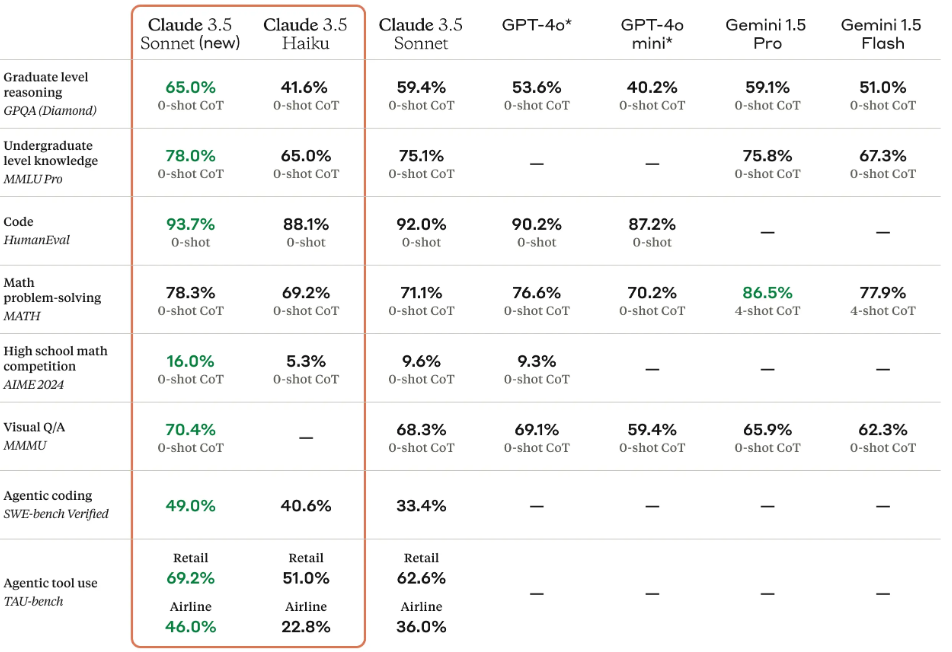
\includegraphics[scale=0.6]{sonnet-comparison.png}
    \caption{Confronto tra \textit{Sonnet} ed altri \gls{llm} - Ottobre 2024}
    \cite{site:updated-sonnet}
    \label{fig:sonnet-comparison}
\end{figure}